\documentclass[12pt]{article}
\usepackage{latexsym}              % symbols
\usepackage{amsmath}               % great math stuff
\usepackage{amssymb}               % great math symbols
\usepackage{amsfonts}              % for blackboard bold, etc
\usepackage{amsthm}                % for theorems
\usepackage{graphicx}              % for insert graph
\usepackage{listings}              % for code block

\lstset{frame=tb,
  language=Java,
  aboveskip=3mm,
  belowskip=3mm,
  showstringspaces=false,
  columns=flexible,
  basicstyle={\small\ttfamily},
  numbers=none,
  numberstyle=\tiny,
  breaklines=true,
  breakatwhitespace=true,
  tabsize=3
}


\newcommand{\N}{\mathbb{N}}
\newcommand{\Z}{\mathbb{Z}}
\newcommand{\R}{\mathbb{R}}
\newcommand{\C}{\mathbb{C}}
\newcommand{\F}{\mathbb{F}}

\renewcommand{\vert}{\,|\,}
\newcommand{\mb}{\textbf}
\newcommand{\norm}[2]{\|{#1}\|_{#2}}
\newcommand{\normm}[1]{\|#1\|}
\newcommand{\bmat}[1]{\begin{bmatrix} #1 \end{bmatrix}}
\newcommand{\pmat}[1]{\begin{pmatrix} #1 \end{pmatrix}}
\newcommand{\eqtext}[1]{\hspace{3mm} \text{#1} \hspace{3mm}}
\newcommand{\set}[1]{\{#1\}}
\newcommand{\inn}[2]{\langle #1, #2 \rangle}
\newcommand{\ra}{\rightarrow}
\newcommand{\Ra}{\Rightarrow}
\newcommand{\tx}[1]{\text{{#1}}}
\newcommand{\abs}[1]{|#1|}
\newcommand{\bigO}{\mathcal{O}}
% \newcommand{\det}{\text{det}}
\DeclareMathOperator{\E}{\mathbb{E}}

\newcommand{\mbt}{\mb t^{(i)}}
\newcommand{\mbx}{\mb x^{(i)}}
\DeclareMathOperator*{\argmax}{arg\,max}
\newcommand{\dd}[2]{\frac{d #1}{d #2}}
\usepackage[margin=0.5in]{geometry}

\begin{document}
  CSC311 A3
  \hfill
  Guanglei Zhu
  \smallskip
  \hrule
  \bigskip
  \begin{enumerate}
    \item \begin{enumerate}
      \item here is the computation graph \\
      \begin{center}
        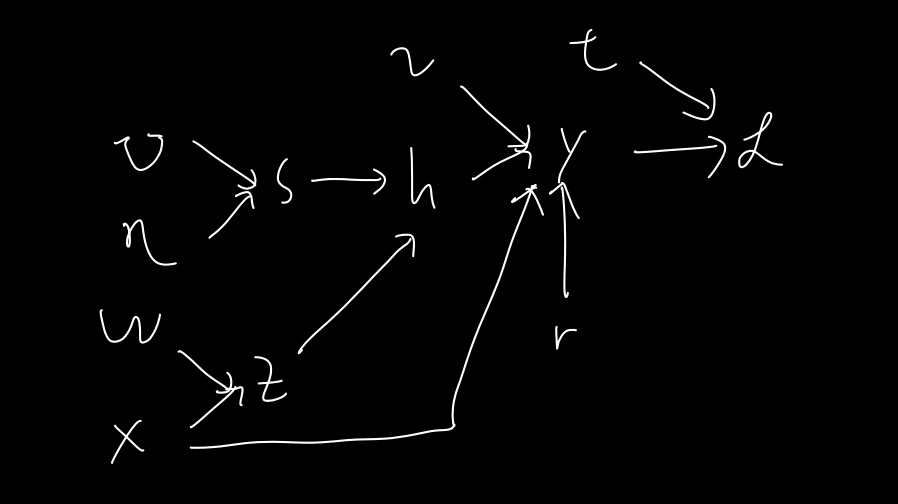
\includegraphics[scale=0.3]{q1.jpg}
      \end{center}
      \item compute all the intermediate quantities, 
      \begin{gather*}
        \overline{\mathcal L} = 1,\, \overline{y} = \overline{\mathcal L} (y-t) = (y-t) \\
        \overline{v_i} = \overline{y} \, h_i ,\, \overline{h_i} = \overline{y} \, v_i,\, 
        \overline{r_i} = \overline{y} \, x_i,\, \dd{y}{x_i}  = \overline{y} \, r_i \\
        \overline{z_i} = \overline{h_i} \, \sigma(s_i),\, \overline{s_i} = \overline{h_i} \, z_i \, \sigma'(s_i) \\
        \overline{W_{ij}} = \overline{z_i} \, x_j ,\, \dd{z_j}{x_i} = W_{ji} \\
        \overline{U_{ij}} = \overline{s_i} \, \eta_j ,\, \overline{\eta_i} = \sum_{j} \overline{s_j} \, U_{ji} \\
        \overline{x_i} = \overline{y} \, r_i + \sum_{j} \overline{z_j} \, \dd{z_j}{x_i} = 
        \overline{y} \, r_i + \sum_{j} \overline{z_j} \, W_{ji}
      \end{gather*}
      after vectorization, we obtain,
      \begin{gather*}
        \overline{\mathcal L} = 1,\, \overline{y} = \overline{\mathcal L} (y-t) = (y-t) \\
        \overline{\mb v} = \overline{y} \, \mb h ,\, \overline{\mb h} = \overline{y} \, \mb v,\, 
        \overline{\mb r} = \overline{y} \, \mb x,\, \dd{y}{\mb x} = \overline{y} \, \mb r \\
        \overline{\mb z} = \overline{\mb h} \odot \sigma(\mb s),\, \overline{\mb s} = \overline{\mb h} \odot \mb z \odot \sigma'(\mb s) \\
        \overline{\mb W} = \overline{\mb z} \cdot \mb x^T ,\, \dd{z_j}{\mb x} = W_j^T \\
        \overline{\mb U} = \overline{\mb s} \cdot \pmb \eta^T ,\, \overline{\pmb \eta} = \mb U^T \cdot \overline{\mb s} \\
        \overline{\mb x} = \overline{y} \, \mb r + \sum_{j} \overline{z_j} \, \dd{z_j}{\mb x} = 
        \overline{y} \, \mb r + \mb W^T \cdot \overline{\mb z}
      \end{gather*}
    \end{enumerate}
    \item \begin{enumerate}
      \item the likelihood function of $\theta, \pi$ is 
      \begin{align*}
        \ell(\pmb \theta, \pmb \pi) &= \sum_{i=1}^N \log p(\mbt, \mbx \vert 
        \pmb \theta, \pmb \pi) \\
        &= \sum_{i=1}^N \log (p(\mbt \vert \pmb \pi) p(\mbx \vert \mbt, \pmb \theta, \pmb \pi)) \\
        &= \sum_{i=1}^N \log p(\mbt \vert \pmb \pi) + 
        \sum_{i=1}^N\sum_{j=1}^{784} \log p(\mbx_j \vert \mbt, \pmb \theta) 
      \end{align*}
    we can maximize these two term seperately, to get $\hat{\pi}_j$ \\
    \begin{align*}
      \sum_{i=1}^N \log p(\mbt \vert \pmb \pi) &= \sum_{i=1}^N \log \prod_{j=0}^9 \pi_j^{t_j^{(i)}}
      = \sum_{i=1}^N \sum_{j=0}^9 t_j^{(i)}\log \pi_j \\
      &= \sum_{i=1}^N (\sum_{j=0}^8 t_j^{(i)}\log \pi_j) + t_9^{(i)} \log (1-\sum_{j=0}^8 \pi_j) 
    \end{align*}
    differentiate with respect to $\pi_k$ for $k \in \{0, \ldots, 8\}$, we get \\
    \[\frac{1}{\pi_k}\sum_{i=1}^N t_k^{(i)} - \frac{1}{\pi_9}\sum_{i=1}^N t_9^{(i)} 
    \overset{\tx{set}}{=} 0 \]
    \[\Longrightarrow \frac{\hat{\pi}_k}{\hat{\pi}_9} = 
      \frac{\sum_{i=1}^N t_k^{(i)}}{\sum_{i=1}^N t_9^{(i)}} \]
    since $\hat{\pi}_i$'s should sum up to 1, as hinted,
    \begin{gather*} \hat{\pi}_9 + 
    \sum_{i=0}^8\hat{\pi}_9\frac{\sum_{i=1}^N t_k^{(i)}}{\sum_{i=1}^N t_9^{(i)}} = 1 \\
    \hat{\pi}_9\,(1 + \frac{1}{\sum_{i=1}^N t_9^{(i)}}\sum_{j=0}^8\sum_{i=1}^N t_j^{(i)}) = 1 \\
    \hat{\pi}_9\,(1 + \frac{1}{\sum_{i=1}^N t_9^{(i)}}(N - \sum_{i=1}^N t_9^{(i)})) = 1 \\
    \Longrightarrow \hat{\pi}_9  = \frac{\sum_{i=1}^N t_9^{(i)}}{N}
    \end{gather*}
    $\forall j \neq 9. \, \hat{\pi}_j = \hat{\pi}_9 \, 
    \frac{\sum_{i=1}^N t_k^{(i)}}{\sum_{i=1}^N t_9^{(i)}} = 
      \frac{1}{N}\sum_{i=1}^N t_j^{(i)}.$ \smallskip \\
    Therefore, $\forall j,$ the MLE of $\pi_j$ is  
    \[\hat{\pi}_j = \frac{1}{N} \sum_{i=1}^N t_j^{(i)} = 
      \frac{\tx{no. of data with label $i$}}{N}. \]
    Use the other term to maximize $\pmb \theta$,
    \begin{align*}
      &\sum_{i=1}^N\sum_{j=1}^{784} \log p(\mbx_j \vert \mbt, \pmb \theta)
      = \sum_{i=1}^N\sum_{j=1}^{784} \sum_{c=0}^9 t_c^{(i)}\log p(\mbx_j \vert \theta_{jc}) \\
      =& \sum_{i=1}^N\sum_{j=1}^{784} \sum_{c=0}^9 t_c^{(i)}
        \log (\theta_{jc}^{x_j^{(i)}}(1-\theta_{jc})^{(1-x_j^{(i)})}) \\
      =& \sum_{i=1}^N\sum_{j=1}^{784} \sum_{c=0}^9 t_c^{(i)} x_j^{(i)}\log \theta_{jc}
      + t_c^{(i)}(1 - x_j^{(i)}) \log (1 - \theta_{jc}) 
    \end{align*}
    differentiate with respect to $\theta_{mn}$, we obtain \\
    \begin{gather*}
      \sum_{i=1}^N t_n^{(i)} x_m^{(i)} \frac{1}{\theta_{mn}} - 
        t_n^{(i)} (1 - x_m^{(i)}) \frac{1}{1-\theta_{mn}} \overset{\tx{set}}{=} 0 \\
      \frac{1}{\theta_{mn}}\sum_{i=1}^N t_n^{(i)} x_m^{(i)} = 
        \frac{1}{1-\theta_{mn}}\sum_{i=1}^N t_n^{(i)} (1 - x_m^{(i)}) \\
      (\frac{1}{\theta_{mn}} - 1)\sum_{i=1}^N t_n^{(i)} x_m^{(i)} = 
        \sum_{i=1}^N t_n^{(i)} (1 - x_m^{(i)}) \\
      \frac{1}{\theta_{mn}} \sum_{i=1}^N t_n^{(i)} x_m^{(i)} = \sum_{i=1}^N t_n^{(i)} \\
      \Longrightarrow \hat{\theta}_{mn} = \frac{\sum_{i=1}^N t_n^{(i)} x_m^{(i)}}{\sum_{i=1}^N t_n^{(i)}}
      = \frac{\tx{no. of data with label $n$ and feature $m$}}{\tx{no. of data with label $n$}}
    \end{gather*}
    \item By Bayes rule, $p(\mb t \vert \mb x, \pmb \theta, \pmb \pi) = 
    \displaystyle\frac{p(\mb x , \mb t \vert \pmb \theta, \pmb \pi)}{\sum_{c=0}^9 p(c)p(\mb x \vert c, \pmb \theta)}
    = \displaystyle\frac{p(\mb t \vert \pmb \pi) p(\mb x \vert \mb t, \pmb \theta)}{\sum_{c=0}^9 p(c)p(\mb x \vert c, \pmb \theta)}$
    so the log likelihood is \\
    \begin{align*}
    & \log p(\mb t \vert \pmb \pi) + \sum_{j=1}^{784} \sum_{c=0}^9 t_c \log p(x_j \vert \theta_{jc}) - 
    \log (\sum_{c=0}^9 p(c) \prod_{j=1}^{784} p(x_j \vert c, \theta_{jc})) \\
    =& \log \pi_c + \sum_{j=1}^{784} \sum_{c=0}^9 t_c (x_j \log \theta_{jc} + (1-x_j) \log (1 - \theta_{jc}))
    - \log (\sum_{c=0}^9 \pi_c \prod_{j=1}^{784} \theta_{jc}^{x_j} (1 - \theta_{jc})^{1 - x_j}) \\
    =& \log \pi_c + \sum_{j=1}^{784} \sum_{c=0}^9 t_c (x_j \log \theta_{jc} + (1-x_j) \log (1 - \theta_{jc}))  \\
    &- \log (\sum_{c=0}^9 \pi_c \, \exp(\sum_{j=1}^{784} (x_j \log \theta_{jc} + (1 - x_j) \log (1 - \theta_{jc})))
    \end{align*}
    (Note: the last line is just for vectorization in coding)
    \item since $\hat{\theta}_{jc}$ could be numerically zero after fitting, $\log (\hat{\theta}_{jc})$ causes
    numerical error and the average log-likelihood could not be computed.
    \newpage
    \item here is the plot of the MLE estimator $\hat{\pmb \theta}$ as 10 separate greyscale images \\
    \begin{center}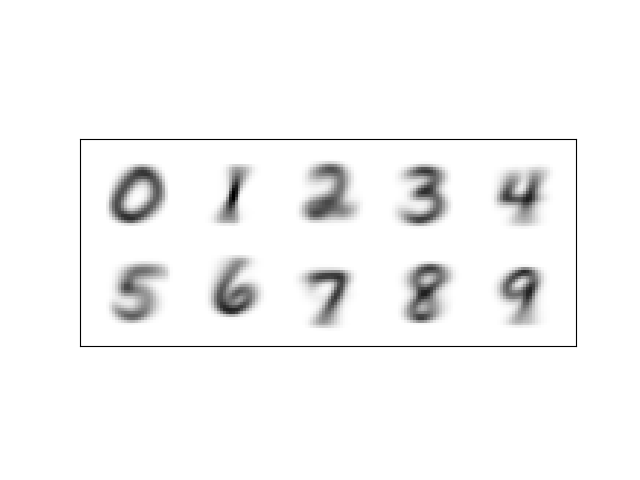
\includegraphics[scale=0.7]{mle.png} \end{center} 
    \item According to MAP estimator, 
    \[\hat{\pmb \theta}_{\tx{MAP}} = \argmax_{\pmb \theta} \log p(\pmb \theta)
    + \log p(\mathcal D \vert \pmb \theta) \]
    where for each $\theta_{jc}, \, \theta_{jc} \sim \tx{Beta}(3, 3)$ \\
    \begin{align*}
      & \argmax_{\pmb \theta} \log \prod_{j, c} p(\theta_{jc})
      + \log \prod_{i=1}^{N} \prod_{j=1}^{784} p(x_j^{(i)} \vert t^{(i)}, \pmb \theta) \\
      =& \argmax_{\pmb \theta} \sum_{j, c} \log \frac{\gamma(3+3)}{\gamma(3)\gamma(3)}
      + (3-1) \log \theta_{jc} + (3-1) \log (1 - \theta_{jc}) 
      + \sum_{i=1}^N \sum_{j=1}^{784} \log p(x_j^{(i)} \vert t^{(i)}, \pmb \theta) \\
      =& \argmax_{\pmb \theta} \sum_{j, c} 2 \log \theta_{jc} + 2 \log (1 - \theta_{jc}) +
      \sum_{i=1}^N\sum_{j=1}^{784} \sum_{c=0}^9 t_c^{(i)} x_j^{(i)}\log \theta_{jc}
      + t_c^{(i)}(1 - x_j^{(i)}) \log (1 - \theta_{jc}) 
    \end{align*}
    differentiate with respect to $\theta_{mn}$, we get 
    \begin{gather*}
      \frac{2}{\theta_{mn}} - \frac{2}{1-\theta_{mn}} + 
      \sum_{i=1}^N t_n^{(i)} x_m^{(i)} \frac{1}{\theta_{mn}} - t_n^{(i)}
      (1-x_m^{(i)})\frac{1}{1-\theta_{mn}} \overset{\tx{set}}{=} 0 \\
      2(1-\theta_{mn}) - 2\theta_{mn} + \sum_{i=1}^N t_n^{(i)} x_m^{(i)} (1-\theta_{mn})
      - t_n^{(i)} (1-x_m^{(i)}) \theta_{mn} = 0 \\
      2 - 4\theta_{mn} + \sum_{i=1}^N t^{(i)}_n x_m^{(i)} - t_n^{(i)} \theta_{mn} = 0 \\
      \hat{\theta}_{mn} = \frac{2 + \sum_{i=1}^N t_n^{(i)} x_m^{(i)}}{4 + \sum_{i=1}^N t_n^{(i)}} 
      = \frac{\tx{2 + no. of data with label $n$ and feature $m$}}
      {\tx{4 + no. of data with label $n$}}
    \end{gather*}
    \newpage
    \item here is the report 
    \begin{center}
\includegraphics[scale=0.5]{q2.jpg} \end{center} 
    \item here is the plot of the MAP estimator $\hat{\pmb \theta}$ as 10 separate greyscale images \\
    \begin{center}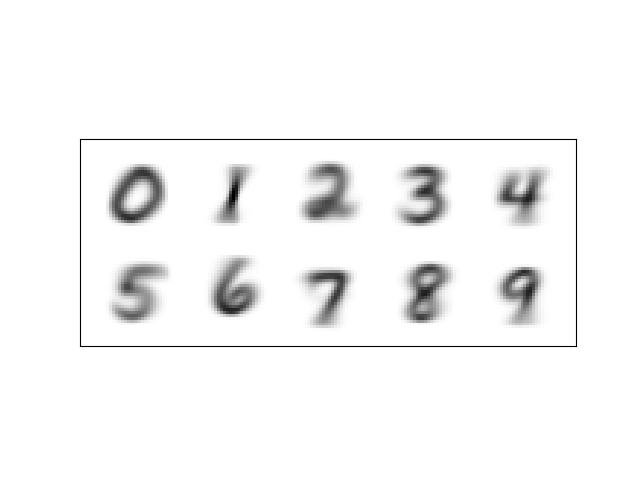
\includegraphics[scale=0.7]{map.png} \end{center} 
    \end{enumerate}
    \item \begin{enumerate}
      \item The posterior $p(\pmb \theta \vert \mathcal D) \propto p(\pmb \theta) p(\mathcal D \vert \pmb \theta)
      \propto \displaystyle\prod_{k=1}^K \theta_k^{a_k - 1} \prod_{i=1}^N p(x^{(i)} \vert \pmb \theta)$
      \begin{align*}
        &= \prod_{k=1}^K \theta_k^{a_k - 1} \prod_{i=1}^N \prod_{k=1}^K \theta_k^{x_k^{(i)}} 
        = \prod_{k=1}^K \theta_k^{a_k - 1} \prod_{k=1}^K \prod_{i=1}^N \theta_k^{x_k^{(i)}} \\ 
        &= \prod_{k=1}^K \theta_k^{a_k - 1} \prod_{k=1}^K \theta_k^{\sum_{i=1}^N x_k^{(i)}} 
        = \prod_{k=1}^K \theta_k^{a_k - 1} \prod_{k=1}^K \theta_k^{N_k} \\
        &= \prod_{k=1}^K \theta_k^{a_k - 1 + N_k}
      \end{align*}
      therefore, $\pmb \theta \vert \mathcal D \sim \tx{Dirichlet}(a_1 + N_1, \ldots, a_K + N_K)$ and 
      Dirichlet distribution is a conjugate prior.
      \item the log-likelihood function of $\pmb \theta$ is 
      \begin{align*}
        \ell(\theta) &= \log p(\mathcal D \vert \mathcal \theta) = \log \prod_{i=1}^N \prod_{k=1}^K \theta_k^{x_k^{(i)}} \\
        &= \sum_{i=1}^N \sum_{k=1}^K x_k^{(i)} \log \theta_k \\
        &= \sum_{i=1}^N \sum_{k=1}^{K-1} x_k^{(i)} \log \theta_k + x_K^{(i)} \log (1-\sum_{k=1}^{K-1} \theta_k)
      \end{align*}
      for $j \neq K$, differentiate with respect to $\theta_j$, we get \\
      \begin{gather*}
        \sum_{i=1}^N x_j^{(i)} \frac{1}{\theta_j} - x_K^{(i)} \frac{1}{\theta_K} \overset{\tx{set}}{=} 0 \\
        \Longrightarrow \hat{\theta}_j = \hat{\theta}_K \frac{\sum_{i=1}^N x_j^{(i)}}{\sum_{i=1}^N x_K^{(i)}} = \hat{\theta}_K \frac{N_j}{N_K}
      \end{gather*}
      since $\hat{\theta}_i$'s should sum up to one, we know
      \begin{gather*}
        \hat{\theta}_K + \hat{\theta}_K \sum_{j=1}^{K-1} \frac{N_j}{N_K} = 1 \\
        \hat{\theta}_K(1 + \frac{1}{N_K} \sum_{j=1}^{K-1} N_j = 1) \\
        \hat{\theta}_K(1 + \frac{1}{N_K} (N - N_K)) = 1 \\
        \Longrightarrow \hat{\theta}_K = \frac{N_K}{N} \tx{ and } \hat{\theta}_j = \frac{N_j}{N}
      \end{gather*}
      thus, the MAP estimate of $\hat{\theta}_i = \frac{N_i}{N}$ for all $i$.
      \item by the posterior predictive distribution, 
      \begin{align*}
         p(x_k^{N+1} = 1 \vert \mathcal D) =& \int p(x_k^{N+1} = 1 \vert \pmb \theta) p(\pmb \theta \vert \mathcal D) \, d \pmb \theta \\
        =& \int \theta_k \prod_{k=1}^K \theta_k^{a_k - 1 + N_k} \, d \pmb \theta \quad (*)
      \end{align*}
      given $\pmb \theta \sim \tx{Dirichlet}(a_1, \ldots, a_K)$, calculate the expectation of $\theta_k$, 
      \[\E(\theta_k) = \int \theta_k p(\pmb \theta) = \int \theta_k \prod_{k=1}^K \theta_k^{a_k - 1} = \frac{a_k}{\sum_{k'} a_{k'}}\]
      let $\pmb \theta \sim \tx{Dirichlet}(a_1 + N_1, \ldots, a_K + N_K)$, observe that 
      \[(*) = \E(\theta_k) = \frac{a_k + N_k}{\sum_{k'} a_{k'} + N_{k'}} = \frac{a_k + N_k}{N + \sum_{k'} a_{k'}}\]
    \end{enumerate}
    \item \begin{enumerate}
      \item here is the report of average conditional log-likelihood:
        \begin{center}
\includegraphics[scale=0.7]{q4a.png} \end{center} 
      \item here is the report of accuracy:
        \begin{center}
\includegraphics[scale=1]{q4b.png} \end{center} 
      \newpage
      \item here is the report of eigenvectors:
        \begin{center}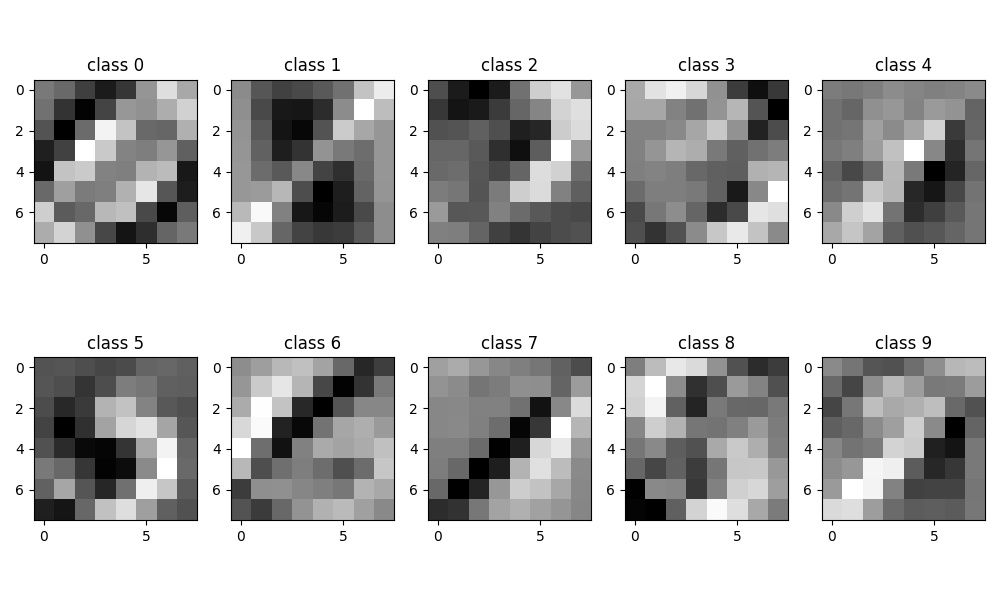
\includegraphics[scale=0.5]{eigenvector.jpg} \end{center} 
    \end{enumerate}
  \end{enumerate}
\end{document}